\section{Aufbau}
Für die Röntgenreflektivitätsmessungen wird ein D8-Labordiffraktometer der Firma 
Bruker-AXS verwendet, siehe Abbildung \ref{fig:Versuchsaufbau}. 
\begin{figure}[H]
    \centering
    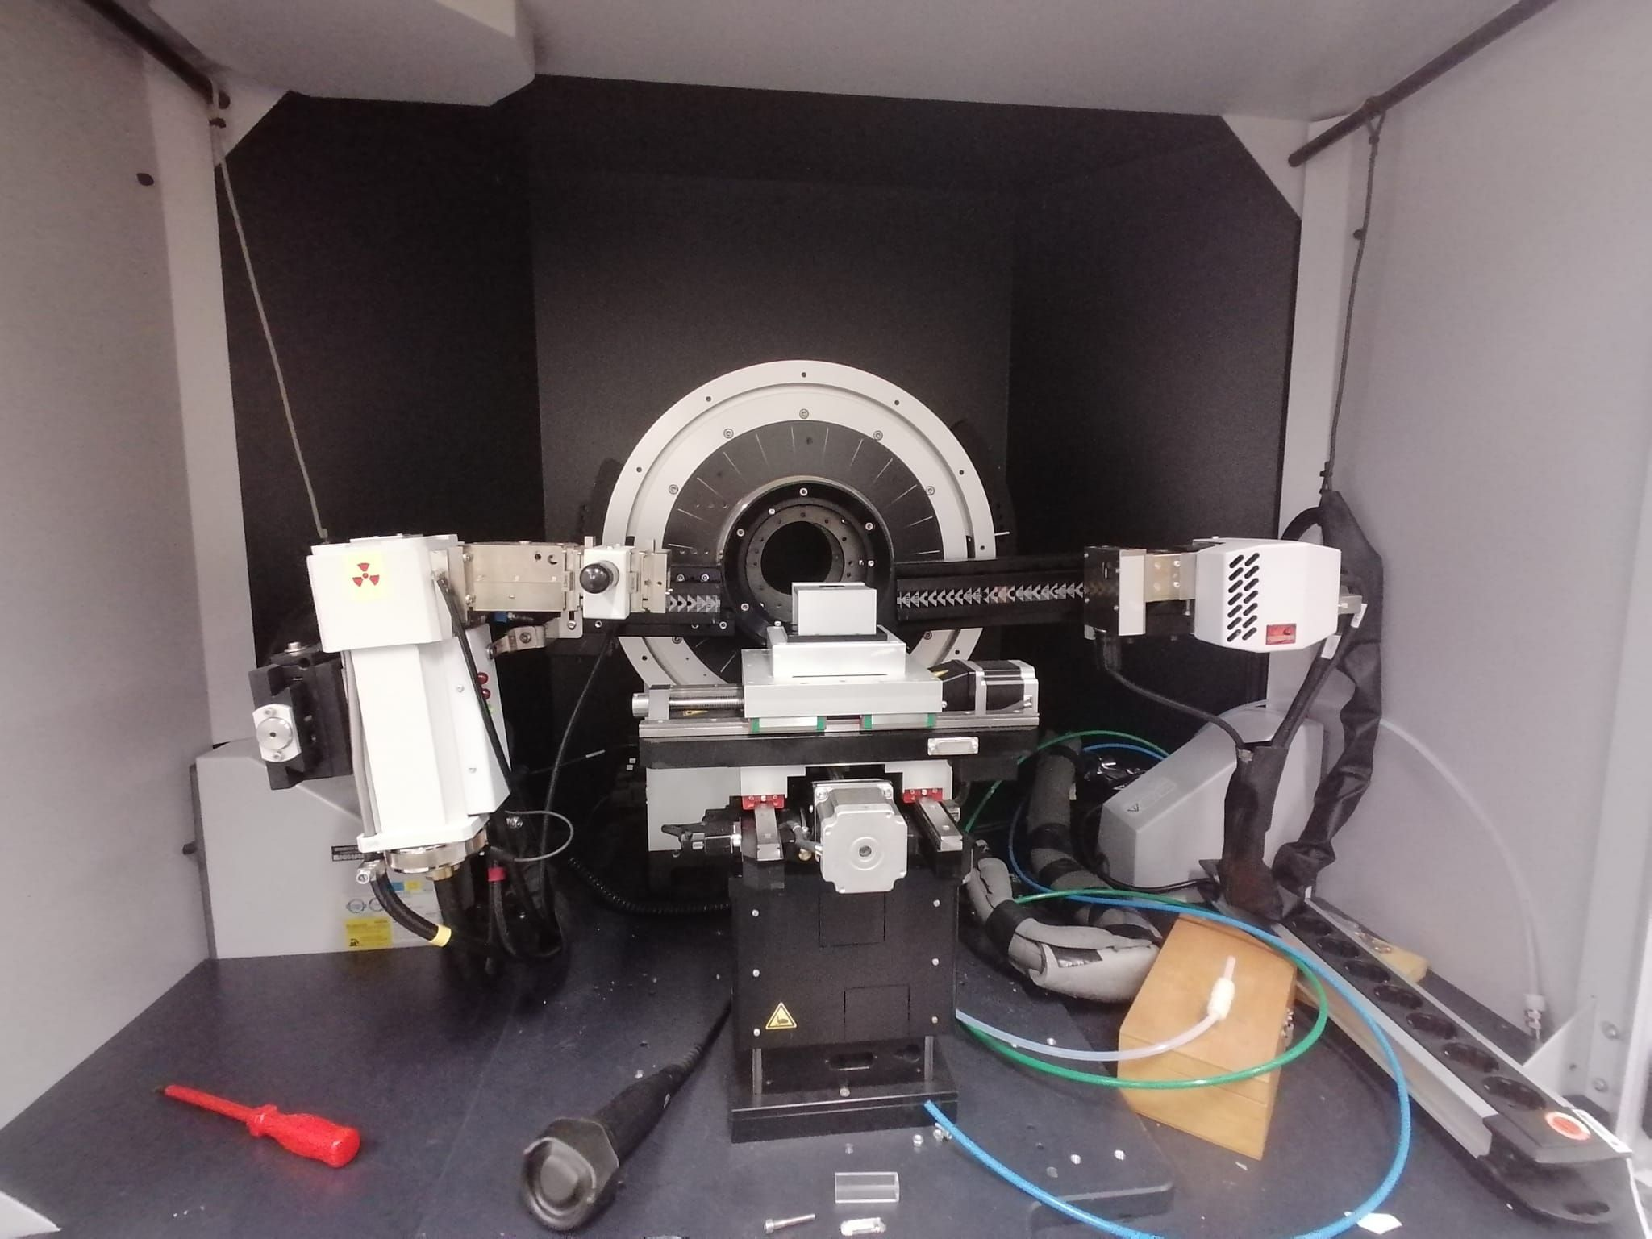
\includegraphics[scale=0.3]{Versuchsaufbau.pdf}
    \caption{Das im Versuch verwendete D8-Labordiffraktometer.}
    \label{fig:Versuchsaufbau}
  \end{figure}
\noindent
In Abbildung \ref{fig:diffraktometer} ist der wesentliche Aufbau 
eines Diffraktometers dargestellt. Es besteht aus einem Probentisch, einer Röntgenröhre
und einem Detektor. Die Röntgenröhre und der Detektor lassen sich um den 
Probentisch drehen. Die genaue Position dieser beiden
kann über das Programm \textit{XRD Commander} eingestellt werden. 
\begin{figure}[H]
  \centering
  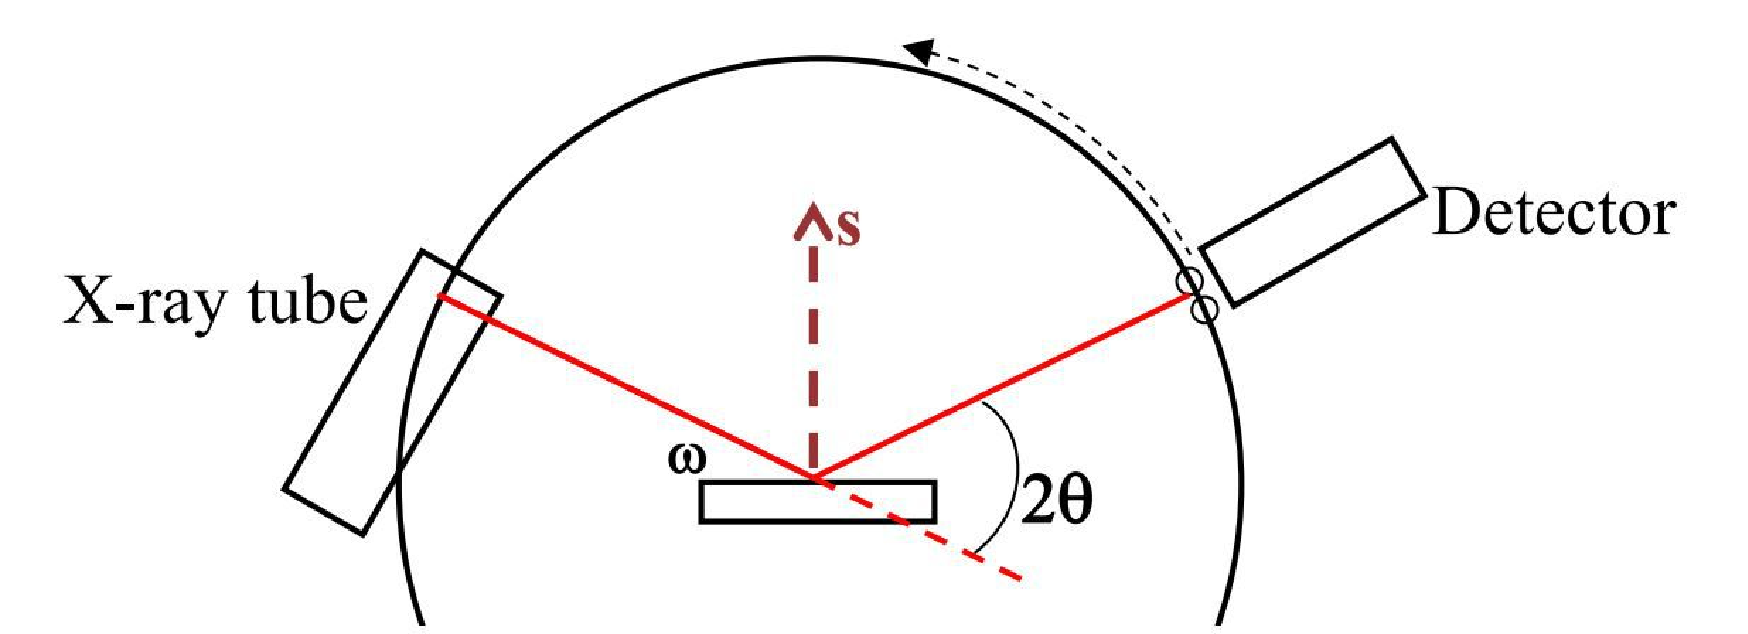
\includegraphics[scale=0.3]{diffraktometer.pdf}
  \caption{Grundlegender Aufbau eines Labordiffraktometers \cite{MIT}.}
  \label{fig:diffraktometer}
\end{figure}
\noindent
Die Röntgenstrahlung wird in der Kupferanodenröhre erzeugt, wobei diese mit einem Strom 
von $35\,\unit{\milli\ampere}$ und einer Spannung von $40\,\unit{\kilo\volt}$ betrieben wird.
Die Strahlung aus der Röntgenröhre wird so ausgerichtet, so dass diese von der zu untersuchende Probe 
in dem Detektor reflektiert wird. Um den Röntgenstrahl zu fokussieren, kann ein Göbelspiegel verwendet werden für präzisere Messungen.
Die Probe, die untersucht wird, besteht aus einem Polystyrolfilm, der auf einem Siliziumwafer (20\,mm × 20\,mm) aufgebracht wurde.

\section{Durchführung}
\subsection{Justierung}
Vor dem eigentlichen Beginn der Reflektivitätsmessung muss die Apparatur durch mehrere Scans 
(Detektorscan, Z-Scan, X-Scan und Rockingscan) justiert werden, 
um sicherzustellen, dass alles richtig ausgerichtet ist.
Es ist wichtig, dass vor der Justierung die Strahlintensität durch einen Autoabsorber reduziert wird, um 
eine Beschädigung des Detektors zu vermeiden.
In Tabelle \ref{tab:Justierung} sind die Messbereiche und weitere Angaben zu den einzelnen Justage-Scans als Orientierung aufgeführt.
Zuerst wird die Probe erstmal aus dem Strahl entfernt, indem die Z-Koordinate geändert wird. Zudem werden die 
Röhre und der Detektor auf 0\,° justiert.
Es wird nun mit einem Detektorscan begonnen, um sicherzugehen, dass der reflektierte Röntgenstrahl zentriert auf den Detektor trifft.
Der resultierende Scan sollte einer Gaußverteilung ähneln und dementsprechend ist das Maximum der Gaußkurve die neue Nullposition.
Danach wird ein Z-Scan durchgeführt, um die Z-Koordinate so anzupassen, dass die Probe die halbe Strahlintensität abdeckt.
Die X-Koordinate wird ähnlich mit einem X-Scan bestimmt, der die Form eines Plateaus mit abgesenkter Intensität besitzt. 
Die Probe ist dann richtig positioniert, wenn die Probe entlang der X-Koordinate 
im Bereich des Strahls liegt. Dabei muss wieder die Hälfte des Eingangsstrahls verdeckt sein.
Sind die X- und Z-Koordinaten justiert und beträgt die Intensität $\frac{1}{2} I\idx{max}$, so wird ein Rocking-Scan durchgeführt.
Des Weiteren soll der Strahl parallel zur Probenoberfläche ausgerichtet werden, deswegen wird ein Rockingscan durchgeführt.
Damit kann eine präzise Justierung der Y-Koordinate garantiert werden und liefert Informationen über die Verkippung der Probe 
zum Strahl. Bei einem Rockingscan rotieren die Röhre und der Detektor um die Probe, wobei 
\begin{equation*}
  \alpha\idx{i} + \alpha\idx{f}= 2\theta
\end{equation*}
gilt. $\alpha\idx{i}$ ist der Einfallswinkel auf die Probe und $\alpha\idx{f}$ der Winkel zwischen Probe und Detektor. Der Y-Scan hat die Form eines symmetrischen Dreiecks. Im Idealfall ist die Nullposition der Peak des Dreiecks.
Sollte das Dreieck nicht symmetrisch sein, muss die Y-Koordinate nochmal nachjustiert werden, so dass die Probe sich im Drehpunkt 
des Diffraktometers befindet. Da der Rockingscan die Position der Probe verändert, 
ist es notwendig, diese anschließend durch einen zweiten Z-Scan wieder in die Mitte des Strahls zu bringen.
Es wird zudem ein weiterer Rockingscan unter den Winkel $2\theta=0,3\,°$ gemacht, um die Justage präziser zu machen.
Darauffolgend ermöglicht ein dritter Z-Scan unter den selben Winkel eine genauere Bestimmung der halben Abschattung, 
da sie direkt aus dem Maximum der Intensitätskurve abgelesen werden kann.
Die Justierung wird mit einem erneuten Rockingscan unter einem höheren Winkel $2\theta=0,5\,°$ beendet.

\begin{table}
    \centering
    \caption{Orientierungswerte für die Justierung \cite{V44}.}
    \label{tab:Justierung}
    \begin{tabular}[t]{l c c c}
    \toprule
    Typ & Messbereich & Schrittweite & Messdauer pro Messpunkt\\
    \midrule
    Detektorscan & -0,5 bis 0,5 & 0,02 & 1\\
    Z-Scan & -1 bis 1 & 0,04 & 1\\
    X-Scan & -20 bis 20 & 1 & 1\\
    Rockingscan $2\theta=0$ & -1 bis 1 & 0,04 & 1\\
    Z-Scan & -0,5 bis 0,5 & 0,02 & 1\\
    Rockingscan $2\theta=0,3$ & 0 bis 0,3 & 0,005 & 1\\
    Z-Scan $2\theta=0,3$ & -0,5 bis 0,5 & 0,02 & 1\\
    Rockingscan $2\theta=0,5$ & 0,2 bis 0,5 & 0,005 & 1\\
    \bottomrule
    \end{tabular}
    \end{table}
%\begin{figure}[H]
%  \centering
%  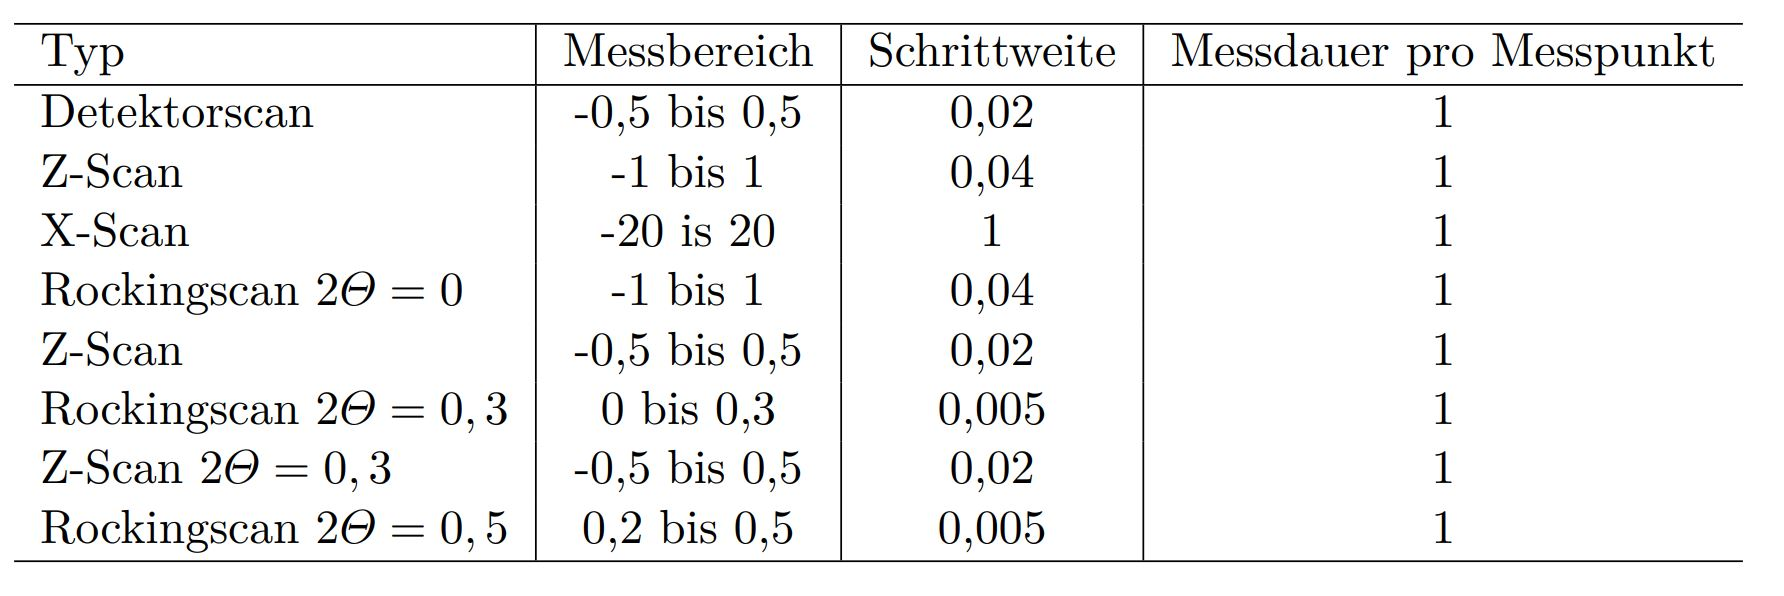
\includegraphics[scale=0.35]{table.JPG}
%  \caption{Orientierungswerte für die Justierung \cite{V44}.}
%  \label{tab:justage}
%\end{figure}

 
\newpage
\subsection{Messung}
Alle erfassten Messdaten werden erst im .raw-Format gespeichert und anschließend 
mithilfe des Programms \textit{File Exchange} in .uxd-Dateien konvertiert, um sie auswerten zu können.

\paragraph{Reflektivitätsscan}
Als erstes wird ein Reflektivitätsscan mit dem Scantyp "Omega/2Theta" aufgenommen. Die Winkel $\omega$ und $2\theta$ sind in 
Abbildung \ref{fig:diffraktometer} eingezeichnet.
Dabei ist der Einfallswinkel $\alpha\idx{i}$ auf die Probe gleich dem Winkel $\alpha\idx{f}$ zwischen Probe und Detektor.
Die Messung wird von 0\,° bis 2,5\,° in 0,005\,°-Schritten durchgeführt.

\paragraph{Diffuser Scan}
Ein Diffuser Scan bestimmt den Anteil der gestreuten Intensität an der Reflektivität. Die "wahre Reflektivität"
kann dann bestimmt werden, indem dieser Scan von dem Reflektivitätsscan abgezogen wird.
Hierfür wird der Detektorwinkel um 0,1\,° gegenüber dem Einfallswinkel verstellt und analog zur ersten Messung gemessen.
Es wird auch den gleichen Scanbereich und Schrittweiten genommen.





